\documentclass[11pt,a4paper]{article}
\PassOptionsToPackage{hyphens}{url}

\usepackage[utf8]{inputenc}
\usepackage[T1]{fontenc}
\usepackage{textcomp}
\usepackage{times}
\usepackage{latexsym}
\usepackage{url}

% Official TACL submission style. The default option is anonymous submission
% with page numbers, rulers, and the confidential TACL header.
\usepackage[]{tacl2021v1}

\usepackage{booktabs}
\usepackage{amsfonts}
\usepackage{amsmath}
\usepackage{amssymb}
\usepackage{microtype}
\usepackage{graphicx}
\usepackage{xcolor}
\usepackage{multirow}
\usepackage{makecell}
\usepackage{enumitem}
\usepackage{array}
\usepackage{dblfloatfix}
\usepackage{float}
\usepackage{placeins}

\Urlmuskip=0mu plus 1mu\relax
\emergencystretch=3em

\raggedbottom
\setcounter{topnumber}{4}
\setcounter{bottomnumber}{2}
\setcounter{totalnumber}{6}
\setcounter{dbltopnumber}{3}
\renewcommand{\topfraction}{0.92}
\renewcommand{\bottomfraction}{0.80}
\renewcommand{\textfraction}{0.07}
\renewcommand{\floatpagefraction}{0.82}
\renewcommand{\dbltopfraction}{0.92}
\renewcommand{\dblfloatpagefraction}{0.82}
\setlength{\dbltextfloatsep}{7pt plus 2pt minus 2pt}
\setlength{\textfloatsep}{7pt plus 2pt minus 2pt}
\setlength{\floatsep}{6pt plus 2pt minus 2pt}
\setlength{\dblfloatsep}{6pt plus 2pt minus 2pt}
\setlength{\intextsep}{7pt plus 2pt minus 2pt}
\setlength{\abovecaptionskip}{4pt}
\setlength{\belowcaptionskip}{0pt}
\renewcommand{\arraystretch}{1.08}
\setlist[itemize]{leftmargin=*,topsep=2pt,itemsep=1.5pt,parsep=0pt,partopsep=0pt}
\setlist[enumerate]{topsep=2pt,itemsep=1pt,parsep=0pt,partopsep=0pt}
\setlength{\abovedisplayskip}{5pt plus 2pt minus 2pt}
\setlength{\belowdisplayskip}{5pt plus 2pt minus 2pt}
\makeatletter
\setlength{\@fptop}{0pt}
\setlength{\@fpbot}{0pt plus 1fil}
\setlength{\@fpsep}{8pt plus 1fil}
\setlength{\@dblfptop}{0pt}
\setlength{\@dblfpbot}{0pt plus 1fil}
\setlength{\@dblfpsep}{8pt plus 1fil}
\makeatother

\newcommand{\num}[1]{#1}
\newcounter{alg}
\newcommand{\algtitle}[1]{\refstepcounter{alg}\textbf{Algorithm~\thealg.}~#1}

\title{Geometric Signatures of Post-Training in LLM Reasoning Trajectories:\\
       Separating Observability from Transferability}

\author{%
  Anonymous TACL submission
}

\begin{document}

\maketitle

\begin{abstract}
Post-training can turn the same pretrained backbone into an instruction
follower, a domain specialist, or a reasoning-distilled model. We ask whether
these variants leave measurable internal traces and whether those traces improve
inference-time decisions. We represent generated-token hidden states as
layer-wise trajectories and summarize their length-residualized correctness
associations in a metric-by-layer geometric signature. We evaluate observability,
candidate-selection utility, and intervention efficacy separately.

In retained retrospective artifacts collected under a fixed prompt, decoder,
and problem slice, matched-width \textsc{Qwen2.5}-derived variants exhibit
different signature matrices. Retrospective bootstrap, budget-sensitivity, and
scale audits reveal recurring contrasts but protocol-sensitive nearest-neighbor
topology; a separately preregistered fresh confirmation chain did not qualify
because of its truncation gate. The signatures are therefore descriptive,
protocol-bounded diagnostics, not universal fingerprints.

Stricter controls change the downstream conclusions. On shared $K{=}8$ candidate
pools, \textsc{GeoVote} (geometric voting) does not improve selection over
majority, length, and likelihood controls. In the locked Qwen-Instruct intervention comparison, every source-derived,
target-calibrated, conventional, sparse, sign-reversed, and matched-random row
has a 95\% paired confidence interval that includes zero relative to no steering. A
separate corrected R1-Distill short-envelope rerun is also null but remains
cap-saturated. Source transfer likewise fails to improve MATH-500, SVAMP, or
long-context evaluations. Among six predeclared label budgets, one
five-label cell reaches $+11$~pp (Holm-adjusted $p{=}0.0443$), but the non-monotone curve does not exhibit a dose--response pattern and is not
presented as a label-efficiency or transfer effect. We
conclude that trajectory geometry provides a protocol-bounded, auditable
measurement of post-training differences; selection utility and transferable
control require separate evidence.
\end{abstract}

\section{Introduction}
\label{sec:intro}

Post-training turns a pretrained language model into a model with a different
behavioral profile.  The same architecture and tokenizer can become a general
instruction follower, a math specialist, or a student distilled from a
reasoning-RL teacher \citep{deepseek-r1-2025}.  These variants are usually
compared at the output: answer accuracy, likelihood, or benchmark score.

Output comparison leaves an internal question open.  Two models may solve the
same problem correctly via different computational paths: a short algebraic
derivation or a longer trace with intermediate checks.  If these behaviors
leave different hidden-state
trajectories, the difference should be measurable before selecting a final
answer or applying an intervention.

We treat measurement and use as separate hypotheses.  For each generated
token, we record the last-position hidden state at every layer.  At one layer,
the resulting sequence is a path through a high-dimensional residual space.  We
summarize that path with a \emph{geometric signature}: a matrix indexed by
trajectory metric and layer.  Each cell is an area under the receiver operating
characteristic curve (AUC) for separating incorrect from correct generations
after log-length residualization.  Values near $0.5$ carry little correctness information;
values farther from $0.5$ indicate a signed association.  We then test the same
trajectory signal at three increasingly demanding evidence levels:
observability, candidate selection, and intervention.  Figure~\ref{fig:overview}
shows the complete protocol.

\begin{figure*}[tbp]
\centering
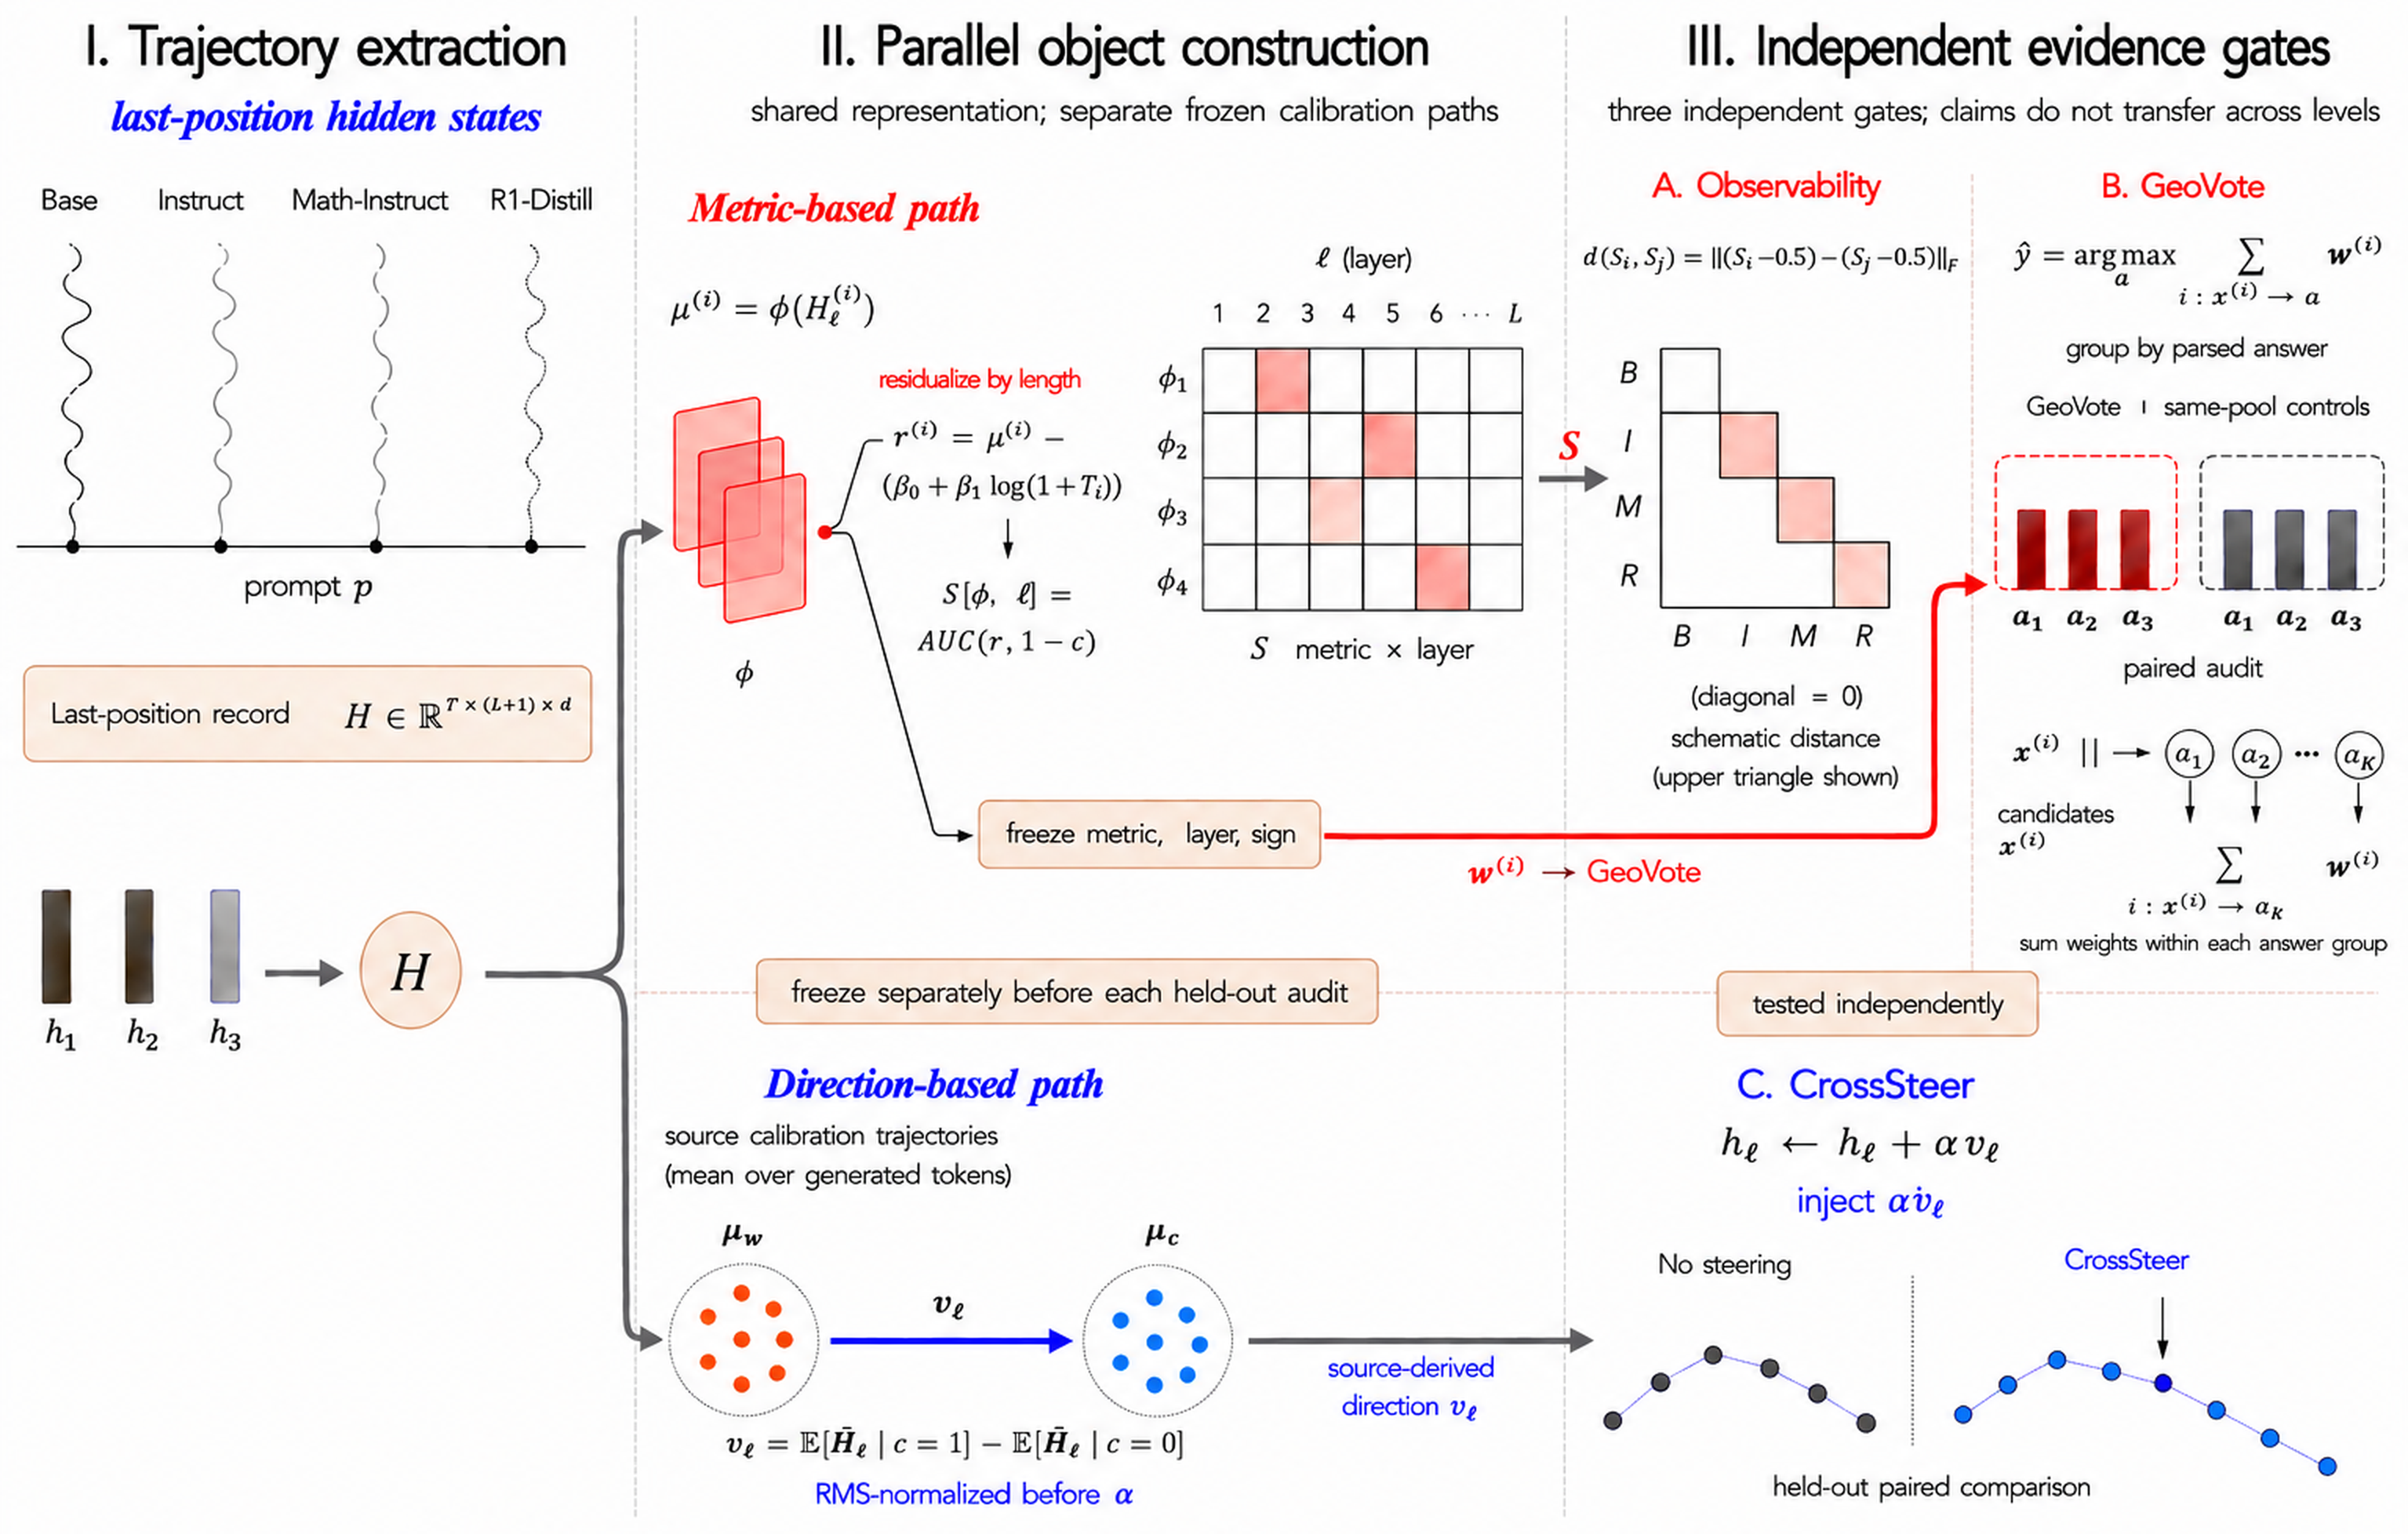
\includegraphics[width=0.88\linewidth]{figures/fig1_overview.png}
\caption{Conceptual overview of the controlled evaluation protocol. Matched
post-training variants share a last-position hidden-state record \(H\), from
which two frozen objects are built on separate calibration paths: a
metric--layer signature \(S\) (length-residualized AUC) and a source direction
\(v_\ell\) (token-mean class difference on \(H\), not on the residual \(r\)).
These objects are tested as three independent evidence gates---observability,
same-pool candidate selection (\textsc{GeoVote}; frozen \(\mu=\phi(H)\)), and
source-direction intervention (\textsc{CrossSteer})---with no cross-level
transfer of claims. Arrows show protocol flow, not a promised gain; matrices,
bars, and trajectories are schematic and do not encode measured results. Each
use is frozen before its own held-out audit.}
\label{fig:overview}
\end{figure*}

\paragraph{First question: is there a measurable association?}
We first use the signature as a diagnostic.  In the retained retrospective
artifacts for a controlled \textsc{Qwen2.5}-derived 1.5B family, the variants
share architecture, tokenizer, prompt, decoding rule, and diagnostic problem
slice.  They differ in
post-training, but they are not treated as a perfectly controlled causal chain.
We therefore ask the narrower question: do their metric--layer correctness
associations differ under the same extraction protocol?  We also audit whether
fine-grained nearest-neighbor relations change with scale and generation budget.
A separately preregistered fresh confirmation chain did not pass its truncation
eligibility gate, so the diagnostic claim remains retrospective and descriptive
(Section~\ref{sec:phenomenon}).

\paragraph{Second question: does the association help at inference time?}
We evaluate two possible uses of a frozen trajectory signal.
\textsc{GeoVote} (geometric voting) inserts a trajectory score into an existing
best-of-$N$ selector.  It is compared with majority voting, output-length
controls, length-residualized scores, and log probability.  \textsc{CrossSteer}
(cross-model steering) constructs a correct-minus-incorrect direction from
calibration trajectories and injects it at a target layer.  We compare source
transfer with target calibration, CAA, ActAdd, SAE activation,
coordinate-sparse, sign-reversed, matched-norm random, and no-steering controls.
All choices are separated into calibration, validation, and locked-test splits.

We distinguish three evidence levels.  An association asks whether geometry
separates correct from incorrect trajectories.  A selection result asks whether
that signal improves a final choice among the same candidates.  An intervention
result asks whether a frozen direction improves a locked target comparison.
A visible geometric difference does not automatically pass the latter two tests;
our claims therefore follow the paired, locked comparisons.

\paragraph{Contributions.}
\begin{itemize}[topsep=2pt,itemsep=2pt,leftmargin=*]
\item We introduce a reproducible protocol that represents each checkpoint by
a metric--layer matrix of length-residualized trajectory--correctness
associations.
\item Retained retrospective artifacts from a matched
\textsc{Qwen2.5}-derived family show different signature matrices under the
fixed protocol.  Bootstrap, budget, and scale audits delimit which descriptive
contrasts recur; a separately preregistered fresh confirmation chain did not
pass its truncation eligibility gate, so no universal or confirmatory
taxonomy claim is made.
\item We introduce and apply a three-level evidence standard that separates
observability from candidate-selection utility and intervention efficacy.
Same-pool controls show that \textsc{GeoVote} adds no reliable selection gain,
and a locked eight-method comparison finds no reliable source-transfer gain.  A
predeclared target-local five-label cell yields $+11$~pp after Holm correction ($p{=}0.0443$);
the complete non-monotone curve bounds the scope of that result.
\end{itemize}

\section{Related Work}
\label{sec:related}

\paragraph{Geometry and dynamics of LLM representations.}
Linear and concept-geometric analyses of hidden states
\citep{park-linear-2023,geiger-causal-2023,anthropic-superposition-2022} usually
study individual activation states.  Dynamical-systems work on recurrent models
\citep{sussillo-barak-2013} instead emphasizes temporal evolution.  We summarize
whole generated hidden-state paths with layerwise functionals, but treat the
result as an extraction-protocol-dependent diagnostic rather than a direct
mechanistic decomposition.

\paragraph{Correctness diagnostics from hidden states.}
Probing and layerwise diagnostic studies
\citep{belinkov-glass-2019,tenney-etal-2019-bert} often use one token or one
layer.  Work on reasoning correctness shows that internal representations can
contain information correlated with whether a chain of thought will succeed
\citep{afzal-etal-2025-knowing}.  Our signature matrix changes the unit of
analysis to a trajectory functional at each layer.  We explicitly distinguish this association evidence from a usable verifier: any final
selection method must beat text, length, likelihood and answer-agreement
controls on the same candidate pool.

\paragraph{Activation steering and transfer.}
Activation addition, representation engineering and inference-time steering are
established tools \citep{turner-steering-2023,panickssery-iti-2024,zou-rep-2023,
todd-function-vectors-2024}.  ActAdd uses a single contrastive prompt pair,
whereas CAA aggregates multiple contrasts \citep{turner-steering-2023,
panickssery-iti-2024}.  Sparse activation steering instead uses a sparse
autoencoder to construct interventions in a sparse latent space
\citep{bayat-etal-2025-sas}.  Separate adaptation lines learn model-specific
interventions with reinforcement learning or reference-free preference
optimization \citep{sinii-etal-2025-steering,wu-etal-2025-reps}.  Those learned,
target-specific training settings answer a different question from our frozen
source-direction transfer at inference time; we cite them as context, rather
than presenting an apples-to-oranges score comparison as a fair baseline.
Steering can be brittle across models and tasks
\citep{tan-etal-2025-steering-off-course}, while cross-model concept-transfer work
suggests that some directions can transfer under appropriate alignment
\citep{huang-etal-2025-cross}.  \textsc{CrossSteer} computes a direction from
full generated trajectories and may apply it across same-width models.  We
compare it directly with target calibration, CAA, ActAdd, SAE-space sparse activation, coordinate-sparse CAA, sign-reversed and
matched-norm random controls; target signature orientation is retained only as a
descriptive covariate, not a transfer guarantee.

\paragraph{OOD arithmetic evaluation.}
Beyond symbolic MATH-500
\citep{hendrycks2021measuring,lightman-verify-2023}, we use the complete SVAMP arithmetic-word-problem
benchmark \citep{patel-etal-2021-nlp} as a separately frozen OOD task.  It is
not selected after observing an intervention result and is reported separately
from MATH-500 rather than pooled with it.

\paragraph{Best-of-$N$ voting.}
Self-consistency \citep{wang-selfconsistency-2023}, likelihood-weighted voting
\citep{xu-etal-2024-soft}, confidence-weighted aggregation
\citep{xu-etal-2025-confidence}, and test-time compute scaling
\citep{snell-tts-2024} use multiple candidates to improve final answers.  Other
inference-time methods exploit layer contrasts directly during decoding, such as
DoLa \citep{chuang-dola-2024}.  \textsc{GeoVote} tests trajectory geometry as a
candidate-level signal, but our controlled audit retains it only as a diagnostic
when length and agreement controls explain its apparent improvement.

\paragraph{Post-training comparisons.}
SFT, preference optimization and reasoning-oriented post-training are commonly
studied through end-task behavior \citep{wei-etal-2022-finetuned,
ouyang-etal-2022-training,rafailov-etal-2023-dpo,deepseek-r1-2025}.  We examine
how matched-width Qwen-derived checkpoints differ in trajectory--correctness
associations, while avoiding a universal taxonomy claim when those associations
change with width, sampling or generation budget.

\section{Framework: Trajectories, Metrics, and the Signature Matrix}
\label{sec:framework}

\subsection{Trajectories}

Given an LLM $f$ with $L$ transformer layers and hidden dimension $d$, a prompt $p$,
and a decoding strategy (greedy unless stated otherwise), we run $f$'s standard
generation loop and record, at every generated token $t \in \{1,\dots,T\}$, the
residual-stream hidden state at every layer
$\ell \in \{0, 1, \dots, L\}$ (index $0$ is the embedding output, $\ell{=}L$ is the
final transformer block). We collect last-position vectors only, giving a tensor
\begin{equation}
\label{eq:trajectory-tensor}
  H \in \mathbb{R}^{T \times (L+1) \times d}.
\end{equation}
A trajectory is one such tensor. The per-layer projection
$H_{:,\ell,:} \in \mathbb{R}^{T\times d}$ is the $\ell$-th \emph{per-layer
trajectory}.

\paragraph{Intuition.} At one fixed layer, this sequence is like tracing a pen
path through a high-dimensional space: each generated token is one point, a
step vector is the short line between adjacent points, and a turning angle asks
whether the path keeps going in the same direction or bends. The metrics below
do not claim that a model literally reasons in Euclidean space; they are compact,
reproducible summaries of how its residual states move while it generates an
answer.  Table~\ref{tab:notation} fixes the notation used below.

\begin{table}[tbp]
\centering
\small
\caption{Notation at a glance. All quantities are fixed before the controlled
evaluations in Section~\ref{sec:crosssteer-no-leakage}.}
\label{tab:notation}
\begin{tabular}{@{}lp{0.67\columnwidth}@{}}
\toprule
Symbol & Meaning \\
\midrule
$p_i, a_i$ & Prompt $i$ and its gold answer \\
$c_i$ & Exact-answer correctness indicator for one generated answer \\
$T, L, d$ & Generated-token count, transformer depth, and hidden width \\
$H^{(i)}$ & Generated-token hidden-state tensor for example $i$ \\
$\phi, S[\phi,\ell]$ & Trajectory function and its metric--layer correctness association \\
$v_\ell, \alpha$ & Layer-$\ell$ steering direction and its root-mean-square (RMS)-scaled strength \\
$I_c, I_v, I_l$ & Disjoint calibration, validation, and locked-test problem IDs \\
$N, K$ & Generic sample count in the algorithm; fixed experimental candidate-pool size \\
\bottomrule
\end{tabular}
\end{table}

\subsection{Geometric metrics}

We compute seven trajectory metrics, each producing a scalar per layer. All
computations use float32 even when $H$ is stored in bfloat16, since the inner
products and norms involved underflow in bfloat16 at $d \ge 1024$.

\paragraph{Length-derived.}
\begin{itemize}
\item $\textsc{TrajLen}(H_\ell) = \sum_{t=1}^{T-1} \lVert H_{t+1,\ell,\cdot} - H_{t,\ell,\cdot}\rVert_2$
\item $\textsc{StepNorm}(H_\ell) = \textsc{TrajLen}(H_\ell) / (T-1)$, the
mean step size. Unlike \textsc{TrajLen}, it does not add a term for every
extra generated token.
\end{itemize}

\paragraph{Curvature-derived.} Let
$v_t = H_{t+1,\ell,\cdot} - H_{t,\ell,\cdot}$ and
\begin{equation}
\label{eq:turning-angle}
\theta_t = \arccos\!\left(
  \frac{v_t \cdot v_{t+1}}{\lVert v_t\rVert_2 \lVert v_{t+1}\rVert_2}
\right)
\end{equation}
denote the discrete turning angle at interior step $t$.
Figure~\ref{fig:curvature-schematic} gives a two-dimensional sketch: a small
turning angle means adjacent displacement vectors point similarly, whereas a
large angle means the path changes direction sharply. The computation itself
uses the original layer-space vectors, not this projection.

\begin{figure*}[tbp]
\centering
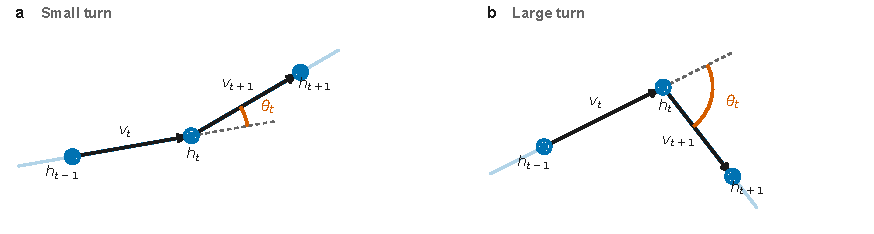
\includegraphics[width=0.78\linewidth]{figures/fig_curvature_schematic.pdf}
\caption{Curvature intuition.  The 2D sketch contrasts small and large turns;
$\theta_t$ is computed from adjacent displacements in the full layer space.}
\label{fig:curvature-schematic}
\end{figure*}

We report $\textsc{CurvMean}$ (the mean of $\theta_t$), $\textsc{CurvVar}$ (sample
variance), and three quantiles $\textsc{CurvMax}$, $\textsc{Curv}_{p90}$,
$\textsc{Curv}_{p99}$. These summarize the distribution of per-step angles
rather than accumulating travel over the whole path. Their sampling behavior can
still depend on how many steps a completion has, so the signature below applies
the same generated-length control to every displayed metric.

\subsection{Geometric signature}

Given a model $f$, a dataset $\mathcal{D}=\{(p_i, a_i)\}$ of prompts and gold
answers, and a correctness indicator $c_i \in \{0,1\}$ for the generated answer
to $p_i$, we define the \emph{geometric signature}
\begin{equation}
\label{eq:signature}
\begin{aligned}
  S(f, \mathcal{D}) &\in [0,1]^{|\Phi|\times (L+1)},\\
  S[\phi, \ell] &= \operatorname{AUC}\bigl(\{\phi(H^{(i)}_\ell)\}_i,\{1-c_i\}_i\bigr),\\
  &\hspace{7em}\phi\in\Phi.
\end{aligned}
\end{equation}
where $H^{(i)}_\ell$ is the per-layer trajectory of $f$ on $p_i$, $\Phi$ is the
fixed set of trajectory functions, and AUC measures how well higher metric
values rank \emph{incorrect} samples above correct ones. We use $1-c_i$ as the
positive label so that interpretation is uniform across functions:
$S[\phi,\ell] > 0.5$ means a high value of $\phi$ flags incorrect outputs;
$S[\phi,\ell]{<}0.5$ indicates the function is sign-flipped (a high value is
associated with correct outputs).

\paragraph{Length-residualized signature.}
Longer completions trivially inflate accumulated path length and can also change
the sampling distribution of per-step statistics. For every metric--layer cell,
we fit a linear nuisance model whose predictor is
$\log(1+\textsc{n-gen-tokens}_i)$, using the diagnostic data, and then compute
the AUC on the residuals. We call this the \emph{length-residualized AUC}; it is
not an AUC restricted to a particular false-positive-rate range. All signature
comparisons in Section~\ref{sec:phenomenon} use this same log-length
residualization. It removes the specified linear component in log length but
does not establish length invariance for nonlinear or extreme-value statistics.

\subsection{Signature distance}
For two signatures we define
\begin{equation}
\label{eq:signature-distance}
  d(S_1, S_2) = \lVert (S_1 - 0.5) - (S_2 - 0.5)\rVert_F,
\end{equation}
so that cells without signal in either model contribute zero. Both signatures must
be computed on the same dataset $\mathcal{D}$. Pairwise $d$ over a model family
yields the distance matrix used in Section~\ref{sec:phenomenon}.

\subsection{Signed orientation}
\label{sec:signed-orientation}

For a single trajectory-function row $\phi$, we also use the signature as a signed diagnostic:
\begin{equation}
\label{eq:signed-orientation}
\begin{split}
\ell^* &= \arg\max_\ell |S[\phi,\ell]-0.5|,\\
o_\phi(f) &= \operatorname{sign}\!\left(S[\phi,\ell^*]-0.5\right).
\end{split}
\end{equation}
Because AUC is computed with incorrect outputs as the positive class,
$o_\phi(f)>0$ means high values of $\phi$ are associated with incorrect generations, while
$o_\phi(f)<0$ means the function is sign-flipped and high values are associated with
correct generations. We record $o_{\textsc{CurvMean}}$ as a descriptive
calibration-time covariate for \textsc{CrossSteer}; it is not a compatibility
rule or a claimed mechanism.  The orientation is learned on labeled calibration
trajectories and then frozen; it is not computed from held-out answers.

\subsection{Inference-time procedures}
\label{sec:inference-procedures}

The diagnostic signature can be used in two logically distinct ways.  Both are
defined here before their controlled evaluations, so that an evaluation result
cannot retroactively change the method definition.

\subsubsection{\textsc{GeoVote}: trajectory-scored aggregation}
\label{sec:geovote-method}

Given a model $f$, a prompt $p$, and $N$ samples $\{x^{(i)}\}_{i=1}^{N}$ produced by
temperature sampling, we extract a per-trajectory scalar
$\mu^{(i)} = \phi(H^{(i)}_{\ell^*})$ for a calibrated trajectory function $\phi$,
layer $\ell^*$, and sign. If calibration says smaller values are more reliable, sample
$i$ receives $w^{(i)}=(\mu^{(i)}+\varepsilon)^{-1}$; otherwise it receives
$w^{(i)}=\max(\mu^{(i)},0)$. The answer string with the largest total weight
is returned:
\begin{equation}
\label{eq:geovote}
\hat{y}=\arg\max_{a}\sum_{i:x^{(i)}\to a}w^{(i)} .
\end{equation}
Aggregation groups candidates by parsed answer and returns the largest total
weight. That combinator is shared with the log-probability-weighted row in
Section~\ref{sec:geovote}; the weight map is not. Frozen \textsc{GeoVote} uses
the sign-dependent weights above, whereas the likelihood control uses
softmax-normalized log-probabilities.
Metric, layer, sign, and aggregation rule are selected on calibration questions
and frozen before held-out evaluation.

\begin{center}
\fbox{\begin{minipage}{0.94\columnwidth}
\small
\algtitle{\textsc{GeoVote}$(p,f,\phi,\ell^*,N)$}\label{alg:geovote}\par
\textbf{Input:} prompt $p$, model $f$, frozen metric $\phi$, layer $\ell^*$,
sign, and sample count $N$.\par
\textbf{1. Freeze.} Select the metric, layer, sign, and vote rule on calibration
questions.  Do not use held-out answers.\par
\textbf{2. Sample and score.} Draw $N$ solutions.  For each solution, extract
$H^{(i)}$, compute $\mu^{(i)}=\phi(H^{(i)}_{\ell^*})$, and convert the signed
score into a nonnegative weight $w^{(i)}$.\par
\textbf{3. Aggregate.} Group candidates by parsed answer and return the answer
with the largest total weight.  Reuse the identical candidate pool for every
comparison rule.\par
\textbf{Output:} one selected answer and the per-candidate audit record.
\end{minipage}}
\end{center}

\subsubsection{\textsc{CrossSteer}: source-direction intervention}
\label{sec:crosssteer-method}

Given a \emph{source} model $f_s$ with trajectories $\{H^{(i)}_{s}\}$ on a dataset
$\mathcal{D}$ with known correctness $\{c_i\}$, define the layer-$\ell$ steering vector
\begin{equation}
\label{eq:crosssteer}
\begin{aligned}
  v_\ell = \mathbb{E}_{i:\,c_i{=}1}\!\bigl[\overline{H^{(i)}_{s,\ell,:}}\bigr]
            - \mathbb{E}_{i:\,c_i{=}0}\!\bigl[\overline{H^{(i)}_{s,\ell,:}}\bigr]
            \in \mathbb{R}^d .
\end{aligned}
\end{equation}
where the inner expectation $\overline{\,\cdot\,}$ averages over the generated tokens
of trajectory $i$. For a target model $f_t$ that shares hidden dimension $d$ with
$f_s$, we run $f_t$'s inference with a forward hook at residual-stream layer $\ell$:
\begin{equation}
\label{eq:crosssteer-injection}
  h_\ell^{f_t}\ \mathrel{+}=\ \alpha\, v_\ell.
\end{equation}
Index $\ell$ runs from $0$ (embedding output) to $L$ (final block output);
injection at $\ell_0{\ge}1$ adds to the residual stream at block
$\ell_0{-}1$'s output, and $\ell_0{=}0$ would add at the embedding output.
Reported cells use $\ell_0\in\{14,20,24\}$.  In the controlled protocol,
the hook is applied only to generated decode steps (never prompt prefilling), and
the direction is RMS-normalized before applying $\alpha$.  Source correctness
labels are used only to build $v_\ell$ on calibration trajectories; held-out
target answers are not used by the hook.  A layer, strength, and schedule may be
chosen only on a disjoint validation split under the predeclared behavior guard,
and are then frozen for one locked evaluation.  This direct form assumes equal
hidden width. Cross-family transfer across different widths would need an
additional learned alignment, which we leave for future work.

\begin{center}
\fbox{\begin{minipage}{0.94\columnwidth}
\small
\algtitle{\textsc{CrossSteer}$(\mathcal{D}_s,f_s,f_t)$}\label{alg:crosssteer}\par
\textbf{Input:} labeled source-calibration trajectories, target-validation
questions, target model $f_t$, and a locked test split.\par
\textbf{1. Build directions.} At each layer, average the source trajectory over
generated tokens and subtract the incorrect mean from the correct mean to obtain
$\{v_\ell\}_{\ell=0}^{L}$.\par
\textbf{2. Freeze.} On disjoint target-validation questions, apply the
predeclared grid rule once to choose layer, RMS-scaled strength, and schedule.
Record the vector hash and freeze the choice.\par
\textbf{3. Intervene.} During target decoding only, add the selected
$\alpha v_\ell$ at the selected layer.  Never modify prompt-prefill states.\par
\textbf{4. Evaluate.} Compare the steered and unsteered outputs problem by
problem on the locked split.  Record accuracy, repairs, breaks, length,
repetition, stopping, and truncation.\par
\textbf{Output:} one locked paired comparison and its complete audit record.
\end{minipage}}
\end{center}

\subsection{Controlled evaluation protocol}
\label{sec:crosssteer-no-leakage}

Any reported steering gain must survive a strict separation between the ids
that supply correctness labels and the ids that supply evaluation labels.  We use
three disjoint splits: source-direction training ids $I_c$, validation ids $I_v$
for the fixed layer/strength/schedule selection rule, and a locked test $I_l$
that is generated exactly once after selection.  Every run records its source
ids, vector hash, model/tokenizer revision, prompt, and resolved decoding
configuration.  A source/evaluation overlap fails automatically and is treated
as exploratory.  On the locked test, comparisons are problem-paired and report
accuracy, repairs, breaks, a paired nonparametric bootstrap confidence interval,
exact paired test, and behavior diagnostics (length, repetition, answer-marker
position, stopping, and truncation).  Multiple formal comparisons receive the
predeclared family-wise correction.  A point estimate without these paired controls is not treated as confirmatory evidence.

\section{Protocol-Dependent Geometric Signatures}
\label{sec:phenomenon}

\subsection{Controlled diagnostic setting}
\label{sec:phenomenon-setting}

We retrospectively compare four matched-width \textsc{Qwen2.5}-derived 1.5B variants
\citep{qwen25-2024,qwen25-math-2024,deepseek-r1-2025}.  They share width,
tokenizer, prompt, decoding rule, and diagnostic problem slice, but they are not
a strict sequence of immediate checkpoints.  Consequently, the comparison asks
whether the checkpoints exhibit different trajectory--correctness associations
under one fixed protocol; it does not identify a unique causal contribution of
any individual post-training operation.
We use SFT for supervised fine-tuning, DPO for direct preference optimization,
and CPT for continued pretraining in Table~\ref{tab:model-lineage}.

\begin{table}[tbp]
\centering
\scriptsize
\setlength{\tabcolsep}{1.5pt}
\caption{Controlled diagnostic family.  Accuracies from the shared retrospective
512-token extraction protocol describe the available correct/incorrect mix;
they are not official benchmark results and are unrelated to the corrected
steering baseline in Section~\ref{sec:crosssteer}.}
\label{tab:model-lineage}
\resizebox{\columnwidth}{!}{%
\begin{tabular}{@{}lllr@{}}
\toprule
Variant & Exact checkpoint & Post-training contrast & Acc. \\
\midrule
\textsc{Base} & Qwen2.5-1.5B & pretraining & 0.37 \\
\textsc{Instruct} & Qwen2.5-1.5B-Instruct & general SFT + DPO & 0.60 \\
\textsc{Math-Instruct} & Qwen2.5-Math-1.5B-Instruct & math CPT/SFT & 0.78 \\
\textsc{R1-Distill} & DeepSeek-R1-Distill-Qwen-1.5B & R1-trace distillation & 0.32 \\
\bottomrule
\end{tabular}%
}
\end{table}

For each model, we extract trajectories on the same 100 GSM8K test problems
(GSM8K IDs 0--99)
\citep{cobbe-etal-2021-training}.  These IDs also form the source-direction
training split in Section~\ref{sec:crosssteer}; the signatures never select a
steering layer, sign, or strength, and steering evaluation uses the disjoint
IDs 100--299.  We compute the seven functionals from
Section~\ref{sec:framework} at all 29 layers, residualize log generated length, and
form one signature matrix $S_i\in[0,1]^{7\times29}$ per checkpoint
(Figure~\ref{fig:phen-heatmap}).

\begin{figure*}[tbp]
\centering
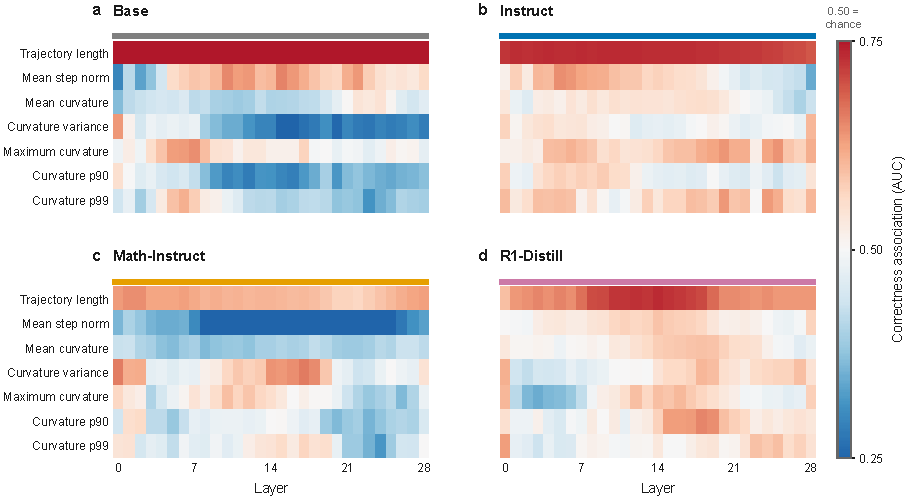
\includegraphics[width=0.98\linewidth]{figures/fig2_signature_heatmaps.pdf}
\caption{Length-residualized metric--layer AUCs for four matched checkpoints;
the shared scale is centered at chance (0.50); the axis label \emph{Mean step
norm} denotes \textsc{StepNorm}.  These are descriptive
associations, not a mechanism, taxonomy, or steering rule.}
\label{fig:phen-heatmap}
\end{figure*}

\subsection{Descriptive distance and its stability boundary}

Table~\ref{tab:phen-distance} gives pairwise distances between centered signature
matrices at the original 512-token budget and a retrospective 2048-token sensitivity comparison;
Figure~\ref{fig:phen-distance-stability} visualizes the paired changes.
The distances are nonzero in both settings, indicating that the checkpoint summaries
differ under each fixed extraction protocol.  The 2048-token artifacts are legacy
retrospective data that do not preserve the full decoder and replay provenance
required by our revision protocol, so this comparison is descriptive and not a
fresh confirmation result.  Their magnitudes change with the
generation budget, and the identity of the largest-distance pair changes, whereas
the closest pair remains \textsc{Instruct}--\textsc{R1-Distill}.  We therefore treat
the distance matrix as a protocol-specific descriptive summary rather than a
protocol-invariant post-training fingerprint.

\begin{table}[tbp]
\centering
\footnotesize
\setlength{\tabcolsep}{5.5pt}
\caption{Pairwise signature distance on the diagnostic GSM8K slice,
$d(S_i,S_j)=\lVert(S_i-0.5)-(S_j-0.5)\rVert_F$.  The 2048-token block is a
retrospective sensitivity comparison using legacy artifacts, not a fresh
confirmation; the closest pair persists while the largest pair changes.}
\label{tab:phen-distance}
\textit{512-token diagnostic}\\[3pt]
\begin{tabular}{@{}lcccc@{}}
\toprule
& \textsc{Base} & \textsc{Inst.} & \textsc{Math} & \textsc{R1} \\
\midrule
\textsc{Base} & 0.00 & 1.83 & 2.63 & 2.13 \\
\textsc{Inst.} & 1.83 & 0.00 & 2.18 & 1.13 \\
\textsc{Math} & 2.63 & 2.18 & 0.00 & 2.09 \\
\textsc{R1} & 2.13 & 1.13 & 2.09 & 0.00 \\
\bottomrule
\end{tabular}\\[7pt]
\textit{2048-token retrospective}\\[3pt]
\begin{tabular}{@{}lcccc@{}}
\toprule
& \textsc{Base} & \textsc{Inst.} & \textsc{Math} & \textsc{R1} \\
\midrule
\textsc{Base} & 0.00 & 1.81 & 2.27 & 2.44 \\
\textsc{Inst.} & 1.81 & 0.00 & 2.06 & 1.54 \\
\textsc{Math} & 2.27 & 2.06 & 0.00 & 1.57 \\
\textsc{R1} & 2.44 & 1.54 & 1.57 & 0.00 \\
\bottomrule
\end{tabular}
\end{table}

\begin{figure*}[tbp]
\centering
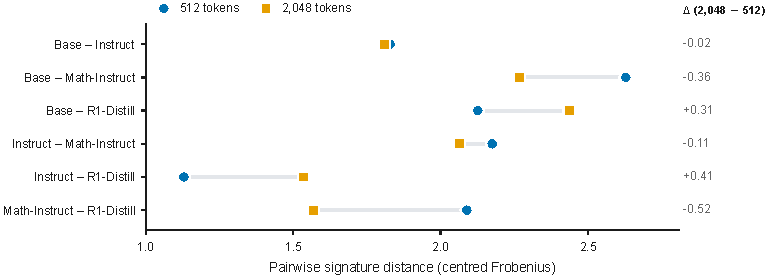
\includegraphics[width=0.88\linewidth]{figures/fig_signature_distance_stability.pdf}
\caption{Pairwise signature distances at 512 and 2,048 tokens; connectors
show within-pair budget change.  This is a descriptive stability audit, not a
model or intervention-selection rule.}
\label{fig:phen-distance-stability}
\end{figure*}

\paragraph{Bootstrap stability audit.}
To quantify the uncertainty behind the displayed nearest-neighbor relations, we
resample shared problem IDs 1,000 times and recompute the directed nearest
neighbor from the matched signature cells.  At 1.5B, Base selects Instruct in
0.631 of resamples, Instruct selects Base in 0.695, and Math selects R1-Distill
in 0.689; the R1-Distill relation is diffuse (Base 0.460, Instruct 0.379).  In
the retrospective 7B audit, Base--R1 and R1--Base are stable (0.993 and 0.995),
whereas Instruct--Base and Math--Base are not (0.506 and 0.512).
These changes have several plausible statistical sources: changing the generation
budget changes stopping and path sampling, changing the slice changes the finite
AUC estimates, and changing scale changes the hidden representation itself.  The
available audits distinguish these sensitivities but do not identify one unique
cause.  We therefore report topology as a stability diagnostic, not as a
post-training explanation.  A separately preregistered fresh confirmation
chain (Qwen 512/2048 and Gemma 512/2048 cells) did not enter confirmatory
analysis because at least one required model in each cell exceeded the
predeclared 25\% truncation ceiling; the signature matrices here are
therefore retained as retrospective, protocol-bounded descriptive evidence,
and the non-qualification is reported rather than treated as evidence about
geometry.  The 25\% ceiling is specific to this confirmatory chain; the
512-token OOD stress envelope in Section~\ref{sec:crosssteer} has a separate
4,096-token low-truncation companion.  The retrospective 7B distance matrix behind the
7B bootstrap numbers is in Appendix~\ref{app:scale-7b} (Table~\ref{tab:scale7b-distance}).

\paragraph{What this supports.}
At 512 tokens, \textsc{Base}--\textsc{Math-Instruct} is the largest displayed
pairwise distance and \textsc{Instruct}--\textsc{R1-Distill} the smallest; at
2048 tokens the smallest pair persists but the largest becomes
\textsc{Base}--\textsc{R1-Distill}.  We therefore
claim only that the matched checkpoints have different metric--layer
correctness-association summaries under the specified protocol.  We do not claim
a stable cluster structure, a universal model fingerprint, or that the distance isolates one
post-training algorithm from all lineage differences.

\paragraph{Localized signals are descriptive hypotheses.}
The heatmaps include localized StepNorm and CurvMean associations, including a
curvature orientation that differs for \textsc{R1-Distill} in this slice.  Such
patterns identify candidate descriptive differences, but they are not used to
choose a target, layer, sign, or strength for an intervention.  The controlled
GeoVote audit in Section~\ref{sec:geovote} and the frozen steering comparison in
Section~\ref{sec:crosssteer} test whether any of these associations provide
utility beyond output-level and activation-steering controls.

\paragraph{Correctness-direction visualization.}
Figure~\ref{fig:phen-separation} projects states onto a direction estimated from
correct and incorrect trajectories in the same model.  It is included solely as
an intuitive visualization of a high-dimensional label-conditioned separation;
it is neither an out-of-sample verifier nor evidence that the corresponding
direction is a causal reasoning mechanism.

\begin{figure*}[tbp]
\centering
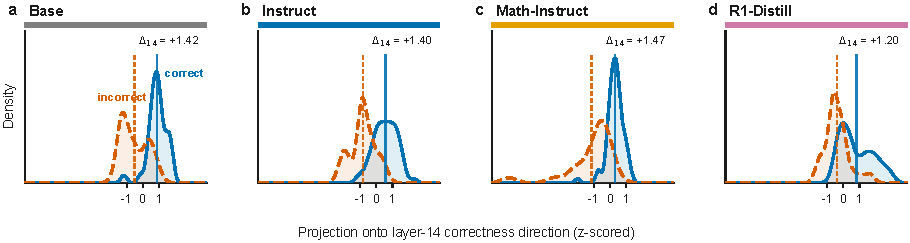
\includegraphics[width=0.98\linewidth]{figures/fig3_correctness_separation.pdf}
\caption{Correct and incorrect generations projected onto each model's
layer-14 correctness direction.  Means are shown after display normalization;
direction and labels come from the same diagnostic split, so the view is
descriptive.}
\label{fig:phen-separation}
\end{figure*}

\section{\textsc{GeoVote}: Does Geometry Improve Candidate Selection?}
\label{sec:geovote}

We reused a frozen, hash-pinned submitted-era historical pool of eight candidate
solutions per question from a 2,048-token sampling run for 50 held-out GSM8K
questions, and applied every selector
to exactly the same candidate pool. This retrospective pool is distinct from
the 512-token diagnostic package in Section~\ref{sec:phenomenon}; its
calibration/held-out halves are documented in
Appendix~\ref{app:geovote-length}. The frozen
GeoVote score is \textsc{StepNorm} at layer 20 with sign $=$ min (smaller
\textsc{StepNorm} receives larger vote weight); the frozen historical vote
weights each candidate by $(\mu+\varepsilon)^{-1}$ and returns the parsed
answer with the largest total weight.
The metric, layer, sign, answer parser, and $K{=}8$ pool were fixed before the
comparison. The question is whether this frozen trajectory score defined in
Section~\ref{sec:geovote-method} adds information beyond answer agreement,
completion length, and likelihood (majority voting is the answer-frequency
control, shortest-output the token-count control).

\subsection{Same-pool length audit}

We evaluate a fixed GSM8K candidate pool on 50 held-out questions; every row
below uses the identical $K{=}8$ candidates, labels, and normalization, and only
the selection/voting score changes.
The trajectory score and its sign are kept fixed. We additionally residualize
that score using calibration data only: for candidate $i$ with score $s_i$ and
$n_i$ generated tokens, we use
$r_i=s_i-(\beta_0+\beta_1\log(1+n_i))$, and the residualized row re-runs the
weighted vote with softmax weights over $r_i$ (larger residualized confidence,
i.e.\ smaller length-adjusted \textsc{StepNorm}, wins).  The raw geometry
picker selects the candidate with the smallest raw \textsc{StepNorm}; the
log-probability-weighted vote applies the same combinator to
softmax-normalized log-probabilities.

\begin{table}[tbp]
\centering
\scriptsize
\setlength{\tabcolsep}{1.0pt}
\caption{Retrospective same-candidate-pool \textsc{GeoVote} audit on 50
held-out GSM8K questions ($K{=}8$).  Every non-majority row is paired against
majority on the identical candidates.  Majority is the text-only
answer-frequency control, and shortest-output is the token-count-only control.
CI is a paired bootstrap interval; R/B denotes repairs/breaks relative to
majority.  Exact $p$ is the paired sign test; $p_{\mathrm{Holm}}$ corrects over
the five non-majority comparisons.}
\label{tab:geovote-audit}
\resizebox{\columnwidth}{!}{%
\begin{tabular}{@{}lrrrrr@{}}
\toprule
Method & acc. & $\Delta$ pp (95\% CI) & R/B & exact $p$ & $p_{\mathrm{H}}$ \\
\midrule
Majority vote & 0.94 & --- & --- & --- & --- \\
Shortest-output control & 0.92 & $-2$ [$-10,+4$] & 1/2 & 1.0000 & 1.0000 \\
Frozen \textsc{GeoVote} & 0.90 & $-4$ [$-10,0$] & 0/2 & 0.5000 & 1.0000 \\
Length-residualized \textsc{GeoVote} & 0.92 & $-2$ [$-10,+4$] & 1/2 & 1.0000 & 1.0000 \\
Raw geometry picker & 0.84 & $-10$ [$-18,-2$] & 0/5 & 0.0625 & 0.2500 \\
Log-probability-weighted vote & 0.82 & $-12$ [$-22,-4$] & 0/6 & 0.0313 & 0.1563 \\
\bottomrule
\end{tabular}%
}
\end{table}

\paragraph{Explicit length-matched null.}
As a stricter control than a scalar residualizer, we form a permutation null on
the same evaluation pool.  Within each question, candidates are sorted by
$(n_{\mathrm{gen}},\mathrm{sample\_idx})$, and the residualized geometry scores
are permuted only within adjacent length pairs.  Across 1,000
predeclared permutations, the mean accuracy is 0.8895 versus the 0.940 majority
baseline (mean paired delta $-5.05$~pp); every permutation is negative, with
paired deltas from $-8$ to $-2$~pp.  Thus a geometry score does not recover
utility even when it is compared within fine-grained length strata; we treat
this as a control-null distribution, not an additional selector.

The central confound is direct: raw geometry confidence has Spearman correlation
$0.830$ with generated length on calibration questions and $0.742$ on the held-out
questions.  Table~\ref{tab:geovote-audit} reports paired uncertainty for every
reported comparator.  Frozen
\textsc{GeoVote} makes no repair and causes two breaks ($-4$ pp, 95\% CI
$[-10,0]$, exact $p=0.50$).  Both the shortest-output control and the
length-residualized rule are $-2$ pp with the same $1/2$ repair/break pattern and
95\% CI $[-10,+4]$.  Thus removing the dominant length relationship does not
recover an advantage over majority voting.  Accordingly, \textsc{GeoVote} is not supported as a reliable inference-time
selector in this setting.

\subsection{Result: association does not imply selection utility}

The result separates diagnostic association from decision utility.  The
length-residualized signatures in Section~\ref{sec:phenomenon} remain measurable,
but their frozen score does not improve the final candidate choice.  We apply the
same standard to intervention: a steering gain must survive locked,
target-calibrated, CAA, ActAdd, sparse, sign-reversed, and matched-random
controls under the protocol in
Section~\ref{sec:crosssteer-no-leakage}.

\section{\textsc{CrossSteer}: Does a Source Direction Transfer?}
\label{sec:crosssteer}

We test whether a correct-minus-incorrect source direction improves a target
model under the frozen protocol in Section~\ref{sec:crosssteer-no-leakage}.
The source direction comes from
\textsc{Qwen2.5-Math}-1.5B-Instruct trajectories (GSM8K IDs 0--99).  The
target is \textsc{Qwen2.5}-1.5B-Instruct, the aligned-orientation boundary
case from the submitted version; \textsc{R1-Distill}, the historical
opposite-orientation repair target, fails its frozen readiness gate under its
model-valid decoder (below).  Selection uses IDs 100--199; the locked test
uses IDs 200--299.  All
methods share the target, greedy decoder, \texttt{decode\_last}
hook, RMS perturbation budget, and problem-indexed baseline, and have the same online form: one RMS-normalized residual-stream vector addition per generated token.  We compare
\textsc{CrossSteer} with target calibration, CAA, ActAdd, SAE sparse activation,
coordinate-sparse CAA, sign reversal, matched random, and no steering; their
offline supervision and online cost are detailed in Appendix~\ref{app:repro} (Table~\ref{tab:steering-budget}).

Selection is allowed only after provenance, EOS, hash, and baseline-parity checks.
Eligible cells must keep the repeated-four-gram increase below $0.05$ and mean
length below $1.5\times$ baseline; validation then selects accuracy with
deterministic ties.  Locked reports include paired uncertainty, repairs/breaks,
length, repetition, truncation, and stop reasons.

We evaluated the R1-Distill target separately with its model-valid 32,768-token sampled
decoder.  Its readiness set contained severe repetition in two outputs
(10\%; 2/20), above the preregistered 5\% ceiling, so we stopped that branch before calibration or intervention.

\subsection{Source transfer versus target labels}

We compare source transfer with target-local supervision at budgets
$0,5,10,20,50,100$.  Budget 0 uses the source vector; nonzero budgets are nested,
hash-selected, class-stratified target subsets.  Layer, strength, decoder, and
locked examples remain fixed.

\begin{table}[tbp]
\centering
\scriptsize
\setlength{\tabcolsep}{2.5pt}
\caption{Frozen target-label-budget curve on GSM8K IDs 200--299.  All rows
use the target-calibrated layer, strength and decoder; label budget 0 uses the
external source vector.  Intervals/tests are paired against the shared 62\%
baseline, with Holm correction over all six rows.}
\label{tab:label-efficiency}
\begin{tabular}{@{}rrrrr@{}}
\toprule
Labels & Acc. & $\Delta$ pp [95\% CI] & R/B & $p_{\mathrm{Holm}}$ \\
\midrule
0 & 0.68 & $+6$ [$-1,+13$] & 9/3 & 0.7300 \\
5 & 0.73 & $+11$ [$+4,+18$] & 13/2 & \textbf{0.0443} \\
10 & 0.64 & $+2$ [$-6,+10$] & 10/8 & 1.0000 \\
20 & 0.63 & $+1$ [$-7,+9$] & 9/8 & 1.0000 \\
50 & 0.67 & $+5$ [$-4,+14$] & 12/7 & 1.0000 \\
100 & 0.65 & $+3$ [$-6,+12$] & 12/9 & 1.0000 \\
\bottomrule
\end{tabular}
\end{table}

\paragraph{Result.}
Table~\ref{tab:label-efficiency} reports the frozen label-budget
curve.  Five target labels give the only corrected positive row: 73\% versus 62\%
baseline ($+11$~pp, 95\% CI $[+4,+18]$, Holm-adjusted $p=0.0443$).  The
zero-label source row is inconclusive (68\%, $+6$~pp, CI $[-1,+13]$), and the
10--100-label rows are non-monotone and non-significant.  The five-label
subset is the single hash-selected, class-stratified subset fixed before
evaluation (calibration indices 6, 39, 66, 73, 80 of target-calibration IDs
100--199); the adjacent 10-label row ($+2$~pp) and the absence
of dose--response indicate that this cell is not a general label-efficiency
effect.  Budget 0 uses the target-calibrated layer and strength, while the
locked family uses
\textsc{CrossSteer}'s own validation-selected values, hence 0.68 vs.\ 0.61.

\subsection{Locked in-domain comparison}
\label{sec:crosssteer-results}

Each eligible method is run once on locked GSM8K IDs 200--299 against a
byte-verified shared baseline, so every delta is problem-paired.

\begin{table*}[tbp]
\centering
\scriptsize
\setlength{\tabcolsep}{4pt}
\caption{Locked Qwen-Instruct GSM8K comparison.  Every row uses the same
baseline and passed the behavior guard; the maximum truncation rate is 6\%.}
\label{tab:crosssteer-locked}
\begin{tabular}{@{}lrrrrrrr@{}}
\toprule
Method & $\ell$ & $\alpha$ & Base acc. & Steered acc. & $\Delta$ pp (95\% CI) & R/B & $p_{\mathrm{Holm}}$ \\
\midrule
ActAdd & 20 & 0.05 & 0.620 & 0.630 & +1.0 [-5.0, +7.0] & 6/5 & 1.0000 \\
CAA & 20 & 0.1 & 0.620 & 0.700 & +8.0 [+0.0, +16.0] & 13/5 & 0.7383 \\
\textsc{CrossSteer} & 14 & 0.025 & 0.620 & 0.610 & -1.0 [-6.0, +4.0] & 3/4 & 1.0000 \\
Matched random & 24 & 0.025 & 0.620 & 0.630 & +1.0 [-2.0, +4.0] & 2/1 & 1.0000 \\
Sign-reversed & 24 & 0.1 & 0.620 & 0.680 & +6.0 [-1.0, +13.0] & 10/4 & 1.0000 \\
SAE sparse & 20 & 0.1 & 0.620 & 0.690 & +7.0 [+0.0, +14.0] & 10/3 & 0.7383 \\
Sparse CAA & 20 & 0.2 & 0.620 & 0.650 & +3.0 [-5.0, +12.0] & 11/8 & 1.0000 \\
Target-calibrated & 20 & 0.1 & 0.620 & 0.650 & +3.0 [-6.0, +12.0] & 12/9 & 1.0000 \\
\bottomrule
\end{tabular}
\end{table*}

\begin{figure*}[tbp]
\centering
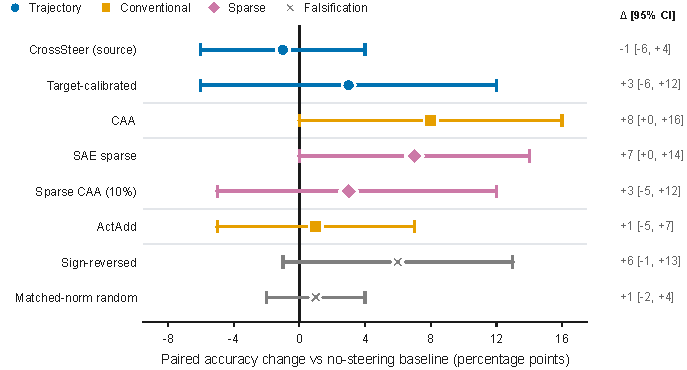
\includegraphics[width=0.88\linewidth]{figures/fig_locked_comparison_forest.pdf}
\caption{Locked GSM8K paired changes from the shared baseline, with 95\%
bootstrap intervals.  Every interval includes zero; source \textsc{CrossSteer}
is slightly negative.}
\label{fig:locked-comparison-forest}
\end{figure*}

\paragraph{Result and behavior controls.}
Table~\ref{tab:crosssteer-locked} and Figure~\ref{fig:locked-comparison-forest}
show that no locked interval excludes zero (the CAA and SAE sparse lower
bounds are exactly 0.0~pp).  CAA and SAE sparse have positive but
underpowered estimates ($+8$ and $+7$~pp; Holm $p=0.74$), whereas source
\textsc{CrossSteer} is $-1$~pp.  Mean-length shifts are small (largest:
\textsc{CrossSteer} $-18.2$ tokens), and repeated-four-gram changes stay within
$\pm0.004$ of the 0.058 baseline, inside the guard.  The comparison therefore supports no source-transfer superiority.  The telemetry
shows no large length or repetition shift that could explain an apparent positive
gain, but it does not identify the mechanism of the null result; complete
per-problem behavior fields will be included in the post-acceptance release.  The sign-reversed control is $+6$~pp, above the positive source direction
but not statistically distinguishable from no steering; rather than
validating the submitted overshoot rule, this indicates that the locked
comparison does not establish directional specificity.  The locked comparison does not establish an advantage; \textsc{CrossSteer}
remains a tested transfer hypothesis rather than a performance winner.

\paragraph{Corrected R1 short-envelope study.}
A corrected greedy 512-token rerun of the submitted R1-Distill setting (same
no-leakage splits, predeclared grid) does not reproduce a reliable gain:
same-target $+3$~pp ($0.41{\to}0.44$, CI $[-8,+14]$, $p{=}0.72$);
cross-source $-1$~pp (CI $[-12,+10]$, $p{=}1.0$).  The corrected baseline
rises from the submitted $0.32$ to $0.41$, confirming that the defective
decoder changed the operating point.  As 85--86\% of completions reached
the generation cap, and the repeated-four-gram fractions were 0.236 (source)
and 0.270 (target calibration) against a corrected baseline of 0.257 (both
shifts within the guard), this rerun audits the
submitted short-budget setting rather than establishing model-valid efficacy.

\subsection{Frozen OOD and long-context tests}

We transfer every eligible frozen configuration, without retuning, to all 500
MATH-500 \citep{hendrycks2021measuring,lightman-verify-2023} and 1,000 SVAMP
problems \citep{patel-etal-2021-nlp}.  MATH-500 uses
\texttt{math-verify==0.9.0}; SVAMP uses a hash-pinned official file and numeric
grader.

\paragraph{OOD result.}
MATH-500 baseline/source accuracies are 33.8/33.2\% ($-0.6$~pp) under a
truncation-heavy 512-token stress envelope.  SVAMP is cleaner (1.9\% baseline
truncation): source \textsc{CrossSteer} reaches 78.7\% versus 80.3\%
($-1.6$~pp, CI $[-3.4,+0.2]$).  The best positive SVAMP estimate, SAE sparse at
$+1.7$~pp, also crosses zero (Holm $p=0.809$).  Neither dataset supports reliable
source transfer (complete rows in Table~\ref{tab:crosssteer-ood}).
A predeclared 4,096-token budget audit of the same
family (Appendix Table~\ref{tab:ood-4096}) confirms the reading: baseline
truncation falls from 45.8\% to 3.2\% and no method shows a reliable paired
gain (all Holm $p{=}1.0$), so the stress envelope does not mask a favorable
higher-budget result.

Long-context tests keep direction, layer, and strength fixed across constant,
prefix, exponential-decay, and relative-RMS schedules at 4,096 and 32,768
tokens.  Source accuracies are 61/61/61/63\% versus the 62\% baseline; all
Holm-adjusted $p$ values are 1.0.  At 32,768 tokens, exponential and relative-RMS
add 311 and 322 mean tokens without improving accuracy.  Target-calibrated
schedules reach 62--66\% but also remain non-significant. Appendix
Table~\ref{tab:long-context} reports every schedule and its token cost. Every
Qwen completion mean stayed far below the caps (largest $\approx$614
tokens; truncation 0--1\%), so neither cap bound (the 4k/32k rows coincide);
these rows test schedule invariance, not bound
long context.

\paragraph{Summary.}
Across locked GSM8K, two OOD datasets, and long-context schedules, the source
direction has no reliable gain.  Only the five-label target-local row survives
correction, supporting a bounded target-alignment result rather than general
source transfer or superiority over conventional steering.

\section{Discussion}
\label{sec:discussion}

\paragraph{What the signature establishes.}
A signature summarizes trajectory--correctness associations under a fixed
model-family, prompt, evaluator, and extraction protocol. Matched Qwen
checkpoints differ under that protocol, but budget and scale audits show that
fine nearest-neighbor topology is neither a universal fingerprint nor a causal
taxonomy.

\paragraph{Association is not mechanism or utility.}
Geometry may reflect planning, formatting, length, termination, confidence, or
unmeasured variables; our controls remove specified confounds, not all causal
alternatives. Association requires a reproducible correct--incorrect difference;
selection requires a same-pool gain over agreement, length, and likelihood;
intervention requires a locked paired gain over fair controls without behavioral
degradation. Evidence at one level does not establish the next.

\paragraph{Implications for transfer.}
Source steering is useful only if it competes with target calibration and
standard activation steering. Under matched target, prompt, split, and budget,
source \textsc{CrossSteer} does not do so. The five-label target-local point is
significant after family-wise correction over the six predeclared label budgets,
but the non-monotone curve is a bounded cell-level result, not a paper-wide
intervention claim or a general sample-efficiency law.

\paragraph{Conclusion.}
Post-training variants can exhibit different length-residualized trajectory
signatures without yielding a useful selector or transferable intervention;
the contribution is a measurement object and an evidence hierarchy that
keeps observability, selection utility, and intervention efficacy distinct.

\section*{Limitations}

The diagnostic uses four matched-width Qwen-derived checkpoints, seven
functionals, and retrospective artifacts. Architecture, scale,
prompt, decoder, stopping, confidence, text style, and nonlinear length effects
may alter it; log-length residualization establishes neither invariance nor a
universal or causal taxonomy. Steering uses a 512-token primary comparison with
separate 4,096/32,768-token audits and a corrected but cap-saturated R1 rerun;
\textsc{GeoVote} remains a same-pool audit, not an independent confidence
signal.

\section*{Artifact Availability}

Upon acceptance, we will release code, configurations, evaluator versions,
content-free per-problem tables, 149 tests, and a CPU smoke test; weights,
benchmark text, and raw hidden states are omitted.

\section*{Ethics Statement}

We use public benchmarks and open-weight models, with no private data;
dual-use steering vectors are withheld until acceptance.


\bibliographystyle{acl_natbib}
\bibliography{references}

\clearpage
\appendix
\raggedbottom
\setlength{\textfloatsep}{5pt plus 1pt minus 1pt}
\setlength{\floatsep}{4pt plus 1pt minus 1pt}
\setlength{\intextsep}{5pt plus 1pt minus 1pt}
\setlength{\abovedisplayskip}{4pt plus 1pt minus 1pt}
\setlength{\belowdisplayskip}{4pt plus 1pt minus 1pt}
\noindent\textbf{Appendix content types.} All appendix material below is
replication detail (TACL Appendix Category~1: configurations, evaluator and
grader versions, statistics and audit protocols) except Tables~8--11, which
are complementary-result tables explicitly referred to from the main text
(TACL Appendix Category~2) and contain no free text beyond their captions.

\section{Reproducibility and Compute (Category 1)}
\label{app:repro}

Each formal run stores a
resolved configuration, model/tokenizer revision, prompt, evaluator version,
randomness policy, git SHA, completion manifest, vector provenance and per-problem
rows.  Directions are fit only on GSM8K IDs 0--99; validation IDs 100--199 and
locked IDs 200--299 are disjoint.  The runner refuses an in-domain evaluation
whose IDs overlap a vector's declared source IDs.

The primary steering result uses deterministic greedy generation. When an
auxiliary best-of-$N$ pool is sampled, its full seed set and the exact candidate
pool are recorded and shared across compared methods. We use $N$ for a generic
algorithmic sample count and $K$ for a fixed experimental pool size; the GeoVote
audit uses $K{=}8$, while the direction-construction audit below uses $K{=}4$
target completions per question. We never choose a highest seed, a single
favorable task, or a post-hoc metric/layer/strength.

One corrected configuration error is disclosed here rather than hidden: an
early steering-runner generation call passed the tokenizer's single EOS id
instead of the Qwen2.5-Instruct model's declared two-id terminator set, which
forced completions toward the generation cap. We corrected the runner,
invalidated the affected run family, and re-ran validation, selection, locked,
OOD, and long-context stages under the model-valid terminator set; no layer,
strength, split, method, prompt, or evaluator was changed to improve an
outcome. The signature matrices, the 2048-token sensitivity comparison, the
7B scale audit, and the \textsc{GeoVote} candidate pool are retained as
retrospective descriptive artifacts rather than fresh confirmatory evidence.

\begin{table*}[tbp]
\centering
\scriptsize
\setlength{\tabcolsep}{3pt}
\caption{Predeclared direction-construction and online-inference budgets for the
Qwen complete-family comparison.  All intervention methods use the same target,
prompt, selected layer/strength grid, RMS rule and \texttt{decode\_last} hook.
The registry records the realized pair count and hashes; no wall-clock ranking is
used to make a scientific claim.}
\label{tab:steering-budget}
\begin{tabular}{@{}p{0.19\linewidth}p{0.49\linewidth}p{0.25\linewidth}@{}}
\toprule
Family & frozen offline direction information & online additional model work \\
\midrule
\textsc{CrossSteer} & 100 source-training questions; source correct--incorrect trajectory means. & One preloaded residual vector add at the selected \texttt{decode\_last} position per generated token. \\
Target-calibrated & 100 target calibration questions; same trajectory construction with target labels. & Same one-vector residual add. \\
CAA / ActAdd / Sparse CAA & 100 source-training questions; $K{=}4$ sampled target completions per question.  CAA averages all valid same-question correct/incorrect pairs; ActAdd uses one SHA-256-selected pair; Sparse CAA applies a fixed 10\% mask to CAA. & Same one-vector residual add. \\
SAE sparse activation & Fixed relative-progress states from the source-training split train the target-local SAE without correctness labels; same-question contrasts determine the frozen feature difference. & Same one-vector residual add. \\
Negative / random / no steering & Exact sign reversal / one predeclared matched-norm seed / no direction; no extra calibration labels beyond the referenced frozen artifact. & Same one-vector residual add / same one-vector residual add / none. \\
\bottomrule
\end{tabular}
\end{table*}

Thus the primary comparison does not give one method an extra online forward
pass, reranking call, online label query, or larger injection budget.  Offline
information differs by construction and is disclosed rather than hidden: the
registry reports source IDs, class counts, completion-row/pair counts, hashes and
vector shape for each method.  The planned post-acceptance code/evidence release includes CPU smoke tests,
split/manifest tests, compact vectors, and provenance artifacts; it will not
redistribute restricted model weights or raw all-layer hidden-state dumps.

\section{Statistical Reporting (Category 1)}
\label{app:statistics}

All steering effects are paired by problem against the baseline generated under
the same frozen prompt and decoder.  We report the paired accuracy delta, a
paired bootstrap confidence interval, an exact paired sign test, and repair/break
counts.  Where several methods are tested in a locked family, the reported
confirmatory $p$ values receive Holm adjustment.  The OOD table is analyzed
separately and is never pooled with GSM8K.

Behavior is part of the endpoint rather than a post-hoc explanation.  Every row
contains generated-token count, content-token count, stop reason, truncation,
repeated four-gram fraction, distinct-$n$ ratios and answer-marker position.  A performance delta without these fields is not considered a complete evaluation artifact.

The long-context chain reused the locked Qwen-Instruct direction, layer,
strength, prompt and greedy decoder and changed only the schedule and the
maximum generated-token budget; each cell is paired with the same 62\%
no-steering baseline on GSM8K IDs 200--299, regenerated under each budget
(mean 292 vs.\ 286 locked tokens).  No cell's mean length exceeded
$\approx$614 tokens and the 4,096-token truncation rates are 0--1\%, so
neither budget cap was binding.

On MATH-500, the SAE-sparse row has a paired interval $[-7.0,-0.2]$~pp whose
exclusion of zero is in the harmful direction, while its Holm-adjusted test
does not survive correction; it is recorded for completeness.

\section{\textsc{GeoVote} Audit Details (Category 1)}
\label{app:geovote-length}

The \textsc{GeoVote} audit in Table~\ref{tab:geovote-audit} uses the
retrospective, hash-pinned 2,048-token pool with $K{=}8$ candidates per question,
using \textsc{StepNorm} at layer 20 with sign $=$ min (smaller
\textsc{StepNorm} receives larger vote weight); the frozen historical vote
weights each candidate by $(\mu+\varepsilon)^{-1}$ and returns the parsed
answer with the largest total weight, while the residualized row re-runs the
weighted vote with softmax weights over the residuals (larger residualized
confidence, i.e.\ smaller length-adjusted \textsc{StepNorm}, receives larger
weight). The pool keeps disjoint calibration
and held-out halves (pool IDs 0--49 and 50--99). Its raw
confidence--length correlations are computed separately on calibration and
held-out questions; the log-length residualizer
$s-(\beta_0+\beta_1\log(1+n_{\mathrm{gen}}))$ is fit on calibration only.
The raw and residualized geometry rows, majority baseline, paired intervals and
exact tests are retained together. Because the result does not improve majority
after the length control, we do not introduce an additional selector or choose
an alternative geometry feature.

\section{Formal Activation-Steering Artifacts (Category 1)}
\label{app:steering-artifacts}

The planned post-acceptance steering registry will contain the source IDs, class counts, source and
target calibration configuration hashes, label hashes, vector hashes and tensor
shape.  CAA uses the mean correct--incorrect prompt-final contrast from the
same-question source pool; ActAdd uses one SHA-256-selected contrast pair; the
SAE sparse activation trains a target-local sparse autoencoder without correctness labels on fixed relative-progress source states, then decodes a same-question sparse feature contrast; the coordinate-sparse ablation applies a fixed 10\% coordinate mask to CAA; a separate negative control is exactly the sign reversal of the source CrossSteer vector.  Each vector is
RMS-normalized before the shared alpha grid.  The validation selector verifies
identical target model, prompt, decoder, evaluation IDs and separately regenerated
baseline rows before it freezes any locked launch.

\section{Frozen OOD Grader Audits (Category 1)}
\label{app:math500-grader}

The formal OOD suite contains all 500 MATH-500 questions and all 1,000 SVAMP
questions. MATH-500 uses \texttt{math-verify==0.9.0}: gold answers are boxed for
extraction, predictions are parsed from the full completion, and symbolic
equivalence decides correctness. Before an OOD launch, the grader audit checks
self-equivalence of all 500 gold answers and fixed positive/negative symbolic
fixtures. SVAMP uses the complete official JSON with a recorded SHA-256, finite
numeric-gold audit, and fixed positive/negative numeric fixtures; it is never
selected after inspecting an intervention delta. Failure to import a required
evaluator, parse a gold answer, or pass a fixture is a hard stop; it cannot
silently fall back to the legacy last-number checker.
\section{Complete Frozen OOD Comparison (Category 2)}
\label{app:ood-results}

\begin{table}[H]
\centering
\scriptsize
\setlength{\tabcolsep}{2.5pt}
\caption{Complete-family OOD evaluation using the GSM8K-selected configuration
without OOD retuning. Cells report accuracy; paired $\Delta$ pp [95\% CI];
Holm-adjusted exact $p$ (correction over the eight-method family per dataset).
MATH-500 and SVAMP baselines are 33.8\% and 80.3\%; baseline truncation is
45.8\% and 1.9\%, respectively. No positive row is significant after Holm
correction.}
\label{tab:crosssteer-ood}
\resizebox{\columnwidth}{!}{%
\begin{tabular}{@{}lcc@{}}
\toprule
Method & MATH-500 & SVAMP \\
\midrule
\textsc{CrossSteer} & 33.2; $-0.6$ [$-3.8,2.6$]; 1.0 & 78.7; $-1.6$ [$-3.4,0.2$]; 0.81 \\
Target-cal. & 33.6; $-0.2$ [$-3.6,3.2$]; 1.0 & 80.6; $+0.3$ [$-1.8,2.4$]; 1.0 \\
CAA & 31.0; $-2.8$ [$-6.6,1.0$]; 1.0 & 79.5; $-0.8$ [$-2.9,1.3$]; 1.0 \\
ActAdd & 31.2; $-2.6$ [$-5.8,0.6$]; 1.0 & 78.7; $-1.6$ [$-3.4,0.2$]; 0.81 \\
Sparse CAA & 32.2; $-1.6$ [$-5.8,2.4$]; 1.0 & 79.3; $-1.0$ [$-3.2,1.2$]; 1.0 \\
Random & 34.8; $+1.0$ [$-1.6,3.8$]; 1.0 & 80.1; $-0.2$ [$-1.6,1.2$]; 1.0 \\
SAE sparse & 30.2; $-3.6$ [$-7.0,-0.2$]; 0.45 & 82.0; $+1.7$ [$-0.3,3.8$]; 0.81 \\
Negative & 33.6; $-0.2$ [$-3.6,3.0$]; 1.0 & 79.7; $-0.6$ [$-2.5,1.3$]; 1.0 \\
\bottomrule
\end{tabular}%
}
\end{table}
\FloatBarrier

\section{Complete 4,096-Token MATH-500 Budget Audit (Category 2)}
\label{app:ood-4096}

\begin{table}[H]
\centering
\scriptsize
\setlength{\tabcolsep}{3pt}
\caption{Complete-family 4,096-token MATH-500 budget audit (predeclared
addendum).  Frozen GSM8K-selected configurations; only the generation budget
changes from the 512-token primary table.  Baseline truncation falls from
45.8\% to 3.2\%, and no row shows a reliable paired gain (all
$p_{\mathrm{Holm}}{=}1.0$).}
\label{tab:ood-4096}
\begin{tabular}{@{}lrrrrr@{}}
\toprule
Method & Acc. & $\Delta$ pp [95\% CI] & R/B & $p_{\mathrm{Holm}}$ \\
\midrule
ActAdd & 0.356 & $-2.6$ [$-6.2,+1.0$] & 35/48 & 1.0000 \\
CAA & 0.356 & $-2.6$ [$-6.4,+1.4$] & 46/59 & 1.0000 \\
\textsc{CrossSteer} & 0.376 & $-0.6$ [$-4.0,+2.8$] & 38/41 & 1.0000 \\
Random & 0.384 & $+0.2$ [$-2.8,+3.2$] & 30/29 & 1.0000 \\
Negative & 0.378 & $-0.4$ [$-4.0,+3.0$] & 38/40 & 1.0000 \\
SAE sparse & 0.358 & $-2.4$ [$-6.4,+1.6$] & 45/57 & 1.0000 \\
Sparse CAA & 0.366 & $-1.6$ [$-6.0,+2.8$] & 57/65 & 1.0000 \\
Target-cal. & 0.402 & $+2.0$ [$-1.8,+5.6$] & 50/40 & 1.0000 \\
\bottomrule
\end{tabular}
\end{table}
\FloatBarrier

\section{Complete Frozen Long-Context Comparison (Category 2)}
\label{app:long-context-results}

\begin{table}[H]
\centering
\scriptsize
\setlength{\tabcolsep}{0.6pt}
\caption{Complete Qwen-Instruct long-context audit.  Accuracy and paired delta
are shown as $4096/32768$-budget pairs; confidence intervals and Holm-adjusted
exact tests are unchanged across the two budgets.  $\Delta$tok is the method
minus baseline mean generated-token change, also shown as $4096/32768$.}
\label{tab:long-context}
\fontsize{6.5}{7.2}\selectfont
\begin{tabular}{@{}llccccc@{}}
\toprule
Dir. & Schedule & Acc. & $\Delta$ pp [CI] & R/B & $p$ & $\Delta$tok; trunc. \\
\midrule
Src. & const. & .61/.61 & $-1$ [$-6,+4$] & 3/4 & 1.000 & $-22.6/-22.6$; 0/0 \\
Src. & exp-1024 & .61/.61 & $-1$ [$-6,+4$] & 3/4 & 1.000 & $+24.4/+311.2$; .01/.01 \\
Src. & pref-256 & .61/.61 & $-1$ [$-6,+4$] & 3/4 & 1.000 & $-18.8/-18.8$; 0/0 \\
Src. & rel-RMS & .63/.63 & $+1$ [$-7,+9$] & 8/7 & 1.000 & $+34.8/+321.5$; .01/.01 \\
Tgt. & const. & .66/.66 & $+4$ [$-5,+13$] & 12/8 & 1.000 & $-19.1/-19.1$; 0/0 \\
Tgt. & exp-1024 & .65/.65 & $+3$ [$-5,+11$] & 10/7 & 1.000 & $-29.5/-29.5$; 0/0 \\
Tgt. & pref-256 & .66/.66 & $+4$ [$-5,+13$] & 12/8 & 1.000 & $-20.1/-20.1$; 0/0 \\
Tgt. & rel-RMS & .62/.62 & $0$ [$-9,+9$] & 11/11 & 1.000 & $-11.4/-11.4$; 0/0 \\
\bottomrule
\end{tabular}
\end{table}

\newpage
\section{Retrospective 7B Scale Audit (Category 2)}
\label{app:scale-7b}

\begin{table}[H]
\centering
\scriptsize
\setlength{\tabcolsep}{3pt}
\caption{Retrospective Qwen-7B pairwise signature distances on GSM8K
$n{=}100$, greedy, max\_new$=512$, reproduced from the submitted-paper scale
replicate.  The matrix is the input to the 7B bootstrap numbers cited in
Section~\ref{sec:phenomenon}; it is the locked 7B pairwise-distance table
\texttt{7b\_pairwise\_signature\_distance.csv} in the post-acceptance
release package, copied verbatim from the submitted-paper extraction
artifacts (pre-correction), and is reported as descriptive stability
evidence only, not as a corrected-generation confirmation run or an
intervention selection rule.}
\label{tab:scale7b-distance}
\begin{tabular}{lrrrr}
\toprule
 & \textsc{Base} & \textsc{Inst.} & \textsc{Math} & \textsc{R1} \\
\midrule
\textsc{Base} & 0.000 & 2.131 & 2.814 & \textbf{0.844} \\
\textsc{Inst.} & 2.131 & 0.000 & 3.076 & 2.198 \\
\textsc{Math} & 2.814 & 3.076 & 0.000 & 2.949 \\
\textsc{R1} & \textbf{0.844} & 2.198 & 2.949 & 0.000 \\
\bottomrule
\end{tabular}
\end{table}



\end{document}
